\chapter{実験}
本章では,人工データ実験を通して提案アプローチの性質調査と実データ解析の結果を述べる.

\section{人工データ実験}
\subsection{シミュレーション}
ニューロン集団のカルシウムイメージングデータをシミュレーションによって作り,解析手法を評価する.
シミュレーションでは1)ニューロンのネットワーク構造を作成し,2)スパイクのシミュレーションを行い,3)蛍光強度の観測データに変換する.
\subsubsection{ネットワーク構造}
シミュレーションに用いるニューロンの個数を$N$として,ニューロンのネットワーク構造を$S \in \{0, 1\}^{N \times N}$とする.
$s_{ij}$はニューロン$i$からニューロン$j$へ活動電位が伝わるかを表している.
本節では$S$の作り方を説明する.

ニューロンのネットワーク構造にはsmall world network\cite{Watts1998}を用いる.
Small world networkはノード数,張り替え確率,初期次数を決めることによってネットワークを作成するアルゴリズムである.
初期次数は,ニューロンが平均何個のニューロンとシナプス結合を持つかという変数である.
張り替え確率は,初期次数によって作成された規則的なグラフのエッジをランダムに張り替える確率である.
そのため,エッジのうち何割が遠くのニューロンとつながっているかを表す変数である.
張り替え確率と初期次数はニューロンのコネクション割合のデータに基づいて決定した.
パラメータ値などは\Secref{sec:Sparam}に記載している.

\subsubsection{スパイクシミュレーション}
スパイクのシミュレーションにIzhikevichモデル~\cite{Izhikevich2003}を用いる.
このモデルはHodgikin-Huxleyモデルをもとにしており,計算コストが低い.
Izhikevichモデルでは,あるニューロンの膜電位が閾値を超えると発火したとみなし,あらかじめ定義したニューロンのネットワーク構造に従って結合を持つニューロンの膜電位を上昇させる.

このシミュレーションで設定しなければいけないのは,個々のニューロンの特徴パラメータ,重み付きのネットワーク構造,外部からのランダムな入力である.
ニューロンの特徴パラメータは\cite{Izhikevich2003}のものを用いた.

重み付きネットワーク構造を$W \in \mathbb{R}^{N \times N}$とすると,ニューロン$i$から$j$へ結合があった場合(つまり$s_{ij} = 1$の場合),$w_{ij}$はニューロン$i$が発火した時にニューロン$j$の膜電位をどれだけ上昇させるかという数値である.
重み付きネットワーク$W$は,前節で作成した$S$の非ゼロ要素を乱数で置き換えることで作成する.
重み付きネットワーク構造$W$の作成方法は2種類ある:
\begin{enumerate}
  \item 全ての重みを同じ分布から生成する
  \item 同じグループへの興奮性ニューロンからの入力は強めにする
\end{enumerate}
具体的な数値については\Secref{sec:spikeparam}に記載している.
1番目の方法で実験を行った際に,重みの大きい別のグループのニューロンからの影響が見られたため,2番目の方法で作り直すことを考えた.

最後に外部からのランダムな入力について説明する.
ニューロンには観測範囲外からの入力がある(以降,外部入力とする).
そのため,シミュレーション中も外部からの電位を乱数としてニューロンの電位に足す.
本論文では同時に活動するニューロンを推定するのが目的の1つであり,ニューロンの活動も外部入力の大きさで表現する.
ある時間帯にあるニューロングループが活動する時,そのニューロングループには平均値を上げた外部入力を足し,それ以外のニューロンには平均$0$の外部入力を足す.
具体的な数値については\Secref{sec:spikeparam}に記載している.
こうすることで,ニューロングループの活動のみ上がる(つまり蛍光強度が上がる).

\subsubsection{カルシウムイメージングモデル}
スパイクデータからカルシウムイオン濃度を計算する~\cite{Vogelstein2009}のモデルを用いる:
\begin{equation}
  [\text{Ca}^{2+}]_{i,t} - [\text{Ca}^{2+}]_{i,t-1} = - \frac{\Delta}{\tau}([\text{Ca}^{2+}]_{i,t-1} - [\text{Ca}^{2+}]_b) + An_{i,t} + \sigma_c \sqrt{\Delta} \epsilon_{i,t}.
  \label{eq:calcium}
\end{equation}
ただし,$[\text{Ca}^{2+}]_{i,t}$をニューロン$i$の時刻$t$でのカルシウムイオン濃度,$[\text{Ca}^{2+}]_b$をカルシウムイオン濃度のベースライン,$\Delta$を時間幅,$\tau$は時定数,$A$は1つのスパイクでのカルシウムイオン濃度の上がり幅,$n_{i,t} \in \{0,1\}$はニューロン$i$の時刻$t$でのスパイク,$\sigma_c$はノイズの分散,$\epsilon_{i,t}$は標準正規分布に従う確率変数である.
この人工データでは,蛍光強度がある値から上昇しない飽和状態は考えないこととする.

次に,同論文のモデルを使ってカルシウムイオン濃度$[\text{Ca}^{2+}]_{i,t}$をカルシウムイメージングで計測される蛍光強度$F_{i,t}$に変換する:
\begin{equation}
	F_{i,t} = \alpha[\text{Ca}^{2+}]_{i,t} + \beta + \sigma_F \epsilon_{i,t}.
  \label{eq:intensity}
\end{equation}
ただし,$\alpha$は強度,$\beta$はバイアス,$\sigma_F$はノイズの分散である.
\Tabref{tab:parameter2}に使用したパラメータを示す.
何種類かの蛍光タンパク質の性能を調べた論文に\cite{Chen2013a}がある.
この論文の,1秒間に10回発火した時のdecay time(蛍光強度が上がり切ってから半分の強度になるまでの時刻)から$\tau = 2.3$とし,SN比から$\sigma_c = 0.5$とした.

\begin{table}[htb]
  \center
  \begin{tabular}{c|c}
		\multicolumn{2}{c}{パラメータ値} \\ \hline
		$[\text{Ca}^{2+}]_b$ & 0.1\\
		$\Delta$ & 0.001\\
		$\tau$ & 2.3\\
		$A$ & 5.0\\
		$\sigma_c$ & 0.5 \\
		$\alpha$ & 1.0\\
		$\beta$ & 10\\
		$\sigma_F$ & 1.0\\ \hline
  \end{tabular}
  \caption{カルシウムイメージングモデルでのパラメータ値}
  \label{tab:parameter2}
\end{table}

\subsubsection{観測モデル}
実データは8[Hz]でサンプリングされたデータなので,シミュレーションした蛍光強度を125[ms]ごとに足し合わせる:
\begin{equation}
  x_{i,t'} = \sum_{t=1}^{125} F_{i,t}.
  \label{eq:observation}
\end{equation}
ここで,$t'$はサンプリング後の時刻を表す.

上記の方法で作成した人工データ時系列と実データをそれぞれ\Figref{fig:art}と\Figref{fig:dat}に示す.
人工データと実データでノイズの乗り方が異なるように見えるが,その理由は分からなかった.
\begin{figure}[htbp]
    \begin{minipage}{0.5\hsize}
			\begin{center}
					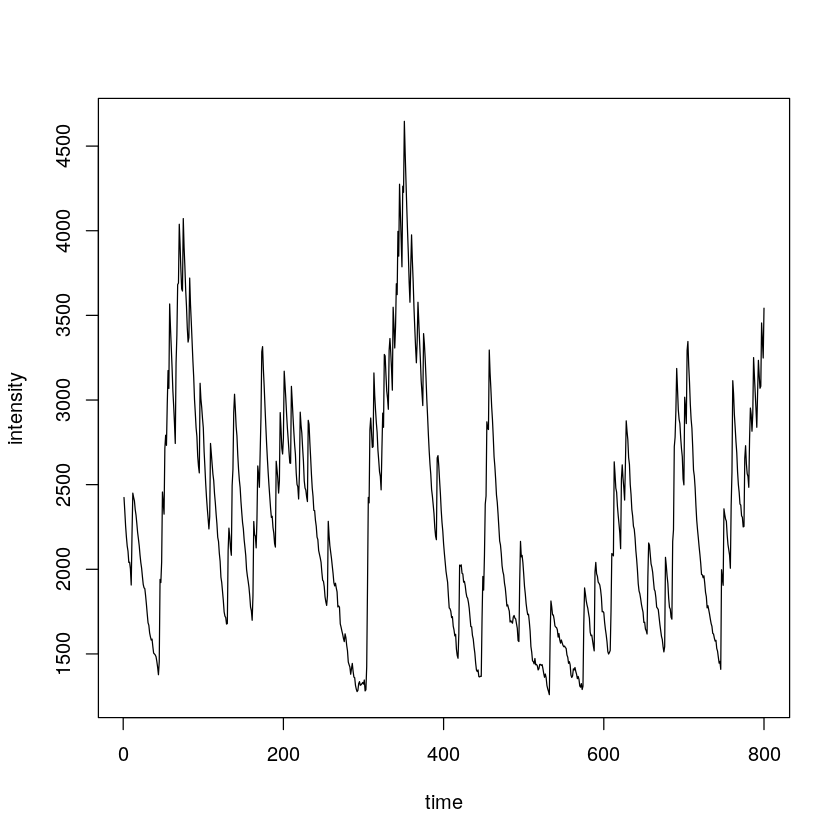
\includegraphics[width=\hsize]{artificial_data}
					\caption{人工データの時系列.}
					\label{fig:art}
			\end{center}
		\end{minipage}
    \begin{minipage}{0.5\hsize}
			\begin{center}
					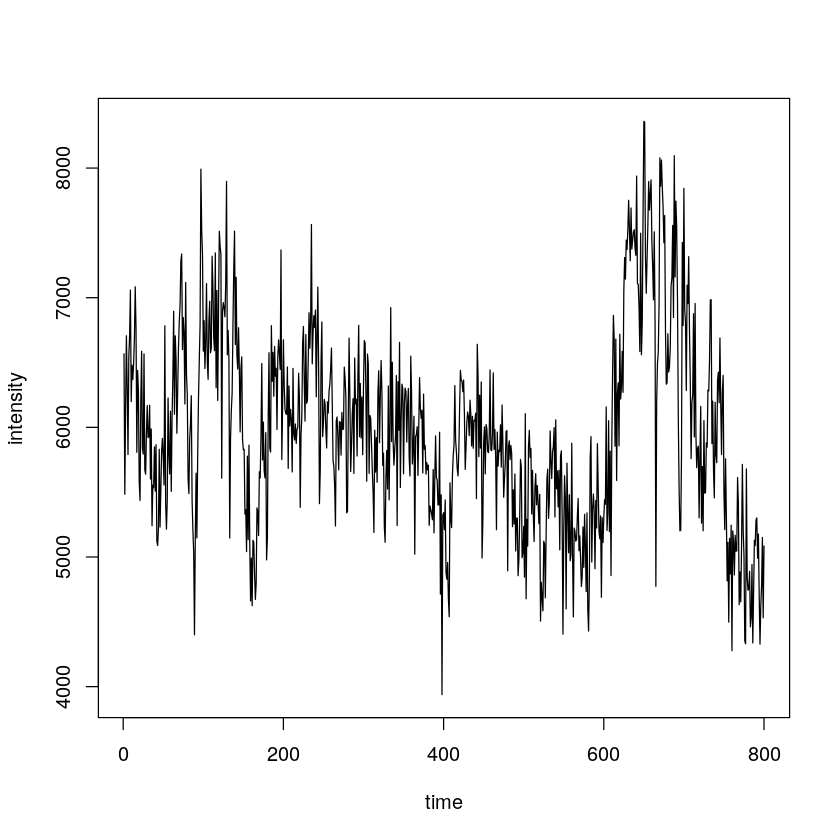
\includegraphics[width=\hsize]{real_data}
					\caption{実データの時系列.}
					\label{fig:dat}
			\end{center}
		\end{minipage}
\end{figure}

\subsubsection{実験設定}
これ以降の実験での共通設定を説明する.
800個の興奮性ニューロンと200個の抑制性ニューロンについてネットワーク構造$S$を作成し,$S$は全実験を通して固定である.
全1000個のニューロンのうち,解析に用いるのは固定された100個の興奮性ニューロンのみとする.
1つのグループに所属するニューロン数は50〜200個とする.
ニューロングループは同時に2つまで活動でき,シミュレーション時間内でどれだけ活動するかは実験によって異なる.
例えば,100[s]のシミュレーションでグループが活動する時間を5[s]とした時に,グループが活動する機会は20回ある.
その20回の内グループが活動できない時間を設定している実験もある.
シミュレーションの安定性から,記載のシミュレーション時間より5[s]長くシミュレーションを行い,最初の5[s]は解析から除外している.

\subsection{$\bar{A}$の推定に関する実験}
本節では$\bar{A}$の推定に関する結果について述べる.
人工データは5[s]ごとに1つか2つのグループが活動するデータを100[s]シミュレーションさせて作成した.
人工データの実験設定は\Tabref{tab:exp1param1}に示す.

隣接行列$\bar{A}$は基底数8から12までをそれぞれ30回ブートストラップを行ってNMFを行った結果を用いる.
NMFの更新則はNesterov更新\cite{Guan2012}を用いる.
NMFは初期値に依存するため,本節では「NMF1回の結果」は「初期値を20回変えてNMFを行い目的関数が最小となった結果」とする.
20回は少ないかもしれないが(1000回ほどこの操作を行っている論文もある),実験サイクルを回すためにこの値にした.
以上のNMFの設定を\Tabref{tab:exp1param2}に示す.

\begin{table}[htb]
  \center
  \begin{tabular}{c|c} \hline
		シミュレーション時間 & 100[s]\\
		グループの活動時間 & 5[s] \\
		グループの活動可能回数 & 20 \\
		$W$の種類 & 1番目 \\
		$Ne_{plus}$ & 0.8 \\
		$Ni_{plus}$ & 0.2\\
		シミュレーション回数 & 100\\ \hline
  \end{tabular}
  \caption{人工データの設定}
  \label{tab:exp1param1}
\end{table}

\begin{table}[htb]
  \center
  \begin{tabular}{c|c} \hline
		1回の結果を出すNMFの回数 & 20 \\
		基底数 & 8 - 12 \\
		ブートストラップサンプル数 & 30 \\
		ブートストラップ方法 & 列のサンプリング \\ \hline
  \end{tabular}
  \caption{NMFの設定}
  \label{tab:exp1param2}
\end{table}

\subsubsection{$\hat{A}(X,K)$の一意性}
前章で述べた通り,NMFには一意性がないため$\hat{A}(X,K)$にも一意性がない.
具体的には,1つの人工データについて初期値のみを変化させてNMFを行うと推定される$\hat{A}(X,K)$は同じではない.
$A$の上三角の要素について$1$と推定された頻度を調べる.
収束性と前章で述べたように寄与率が$D$の空間で取りうる値の範囲を狭めるため,$C$の行和を1とする制約を入れている.
$X$に正規化を加えなかった結果を\Figref{fig:without_scale_A}に,$X$に行和$1$の正規化を加えた結果を\Figref{fig:with_scale_A}に示す.
$X$に行和$1$の正規化を加えると,$D$の自由度は下がるはずである.

\begin{figure}[htbp]
    \begin{minipage}{0.5\hsize}
			\begin{center}
					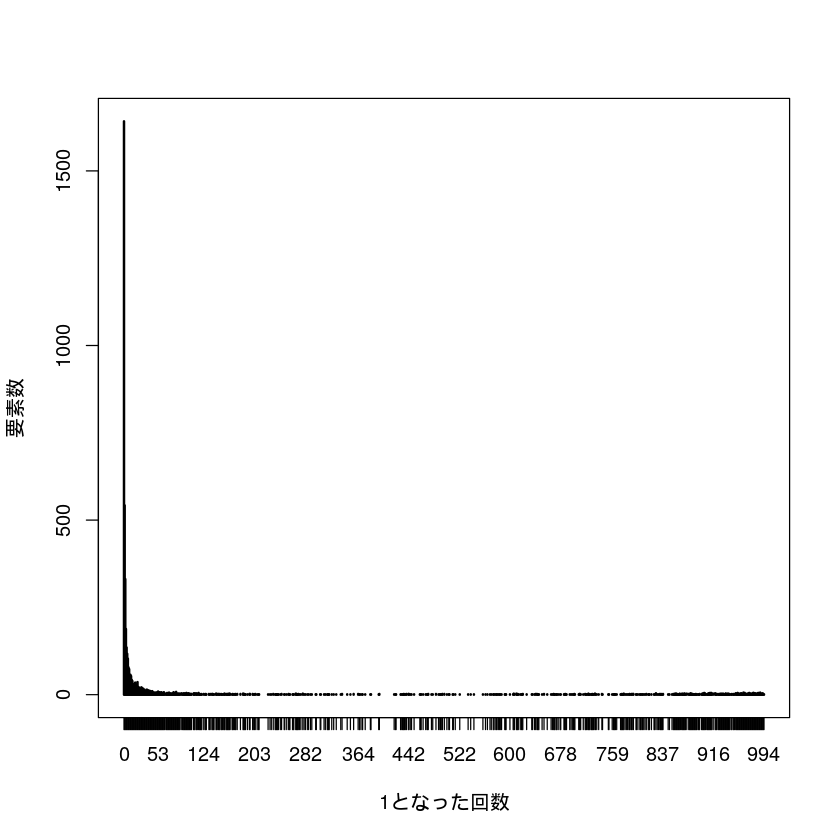
\includegraphics[width=\hsize]{without_scale_A}
					\caption{$X$を正規化せずに初期値を1000回変化させてNMFから$\hat{A}(X,K)$を推定し,各要素について$1$と推定された頻度.}
					\label{fig:without_scale_A}
			\end{center}
		\end{minipage}
    \begin{minipage}{0.5\hsize}
			\begin{center}
					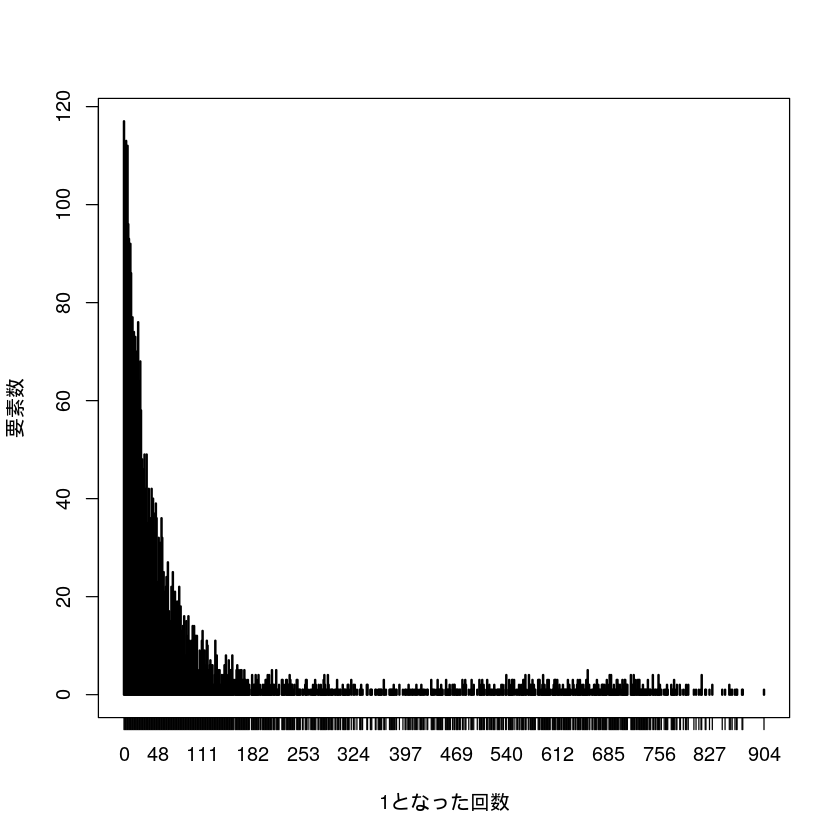
\includegraphics[width=\hsize]{with_scale_A}
					\caption{$X$を行和$1$で正規化して初期値を1000回変化させてNMFから$\hat{A}(X,K)$を推定し,各要素について$1$と推定された頻度.}
					\label{fig:with_scale_A}
			\end{center}
		\end{minipage}
\end{figure}

$\hat{A}(X,K)$に一意性がある場合は,ある$\hat{A}(X,K)$の要素が$1$と推定される回数は$0$か$1000$になる.
結果より,そのようになっていないので$\hat{A}(X,K)$に一意性がないのがわかる.
また,\Figref{fig:with_scale_A}より$X$を正規化しない方がばらつきが小さい.
これは,正規化をしない方が$X$の中の大きな値に推定が引っ張られ,同じ局所解に陥りやすくなっているからだと考えられる.

\subsubsection{NMFを用いる妥当性}
NMFを用いて隣接行列を求める性能を検証するため,NMF,PCA,ICA,logistic regression,glassoの性能の比較を行った.
Logistic regressionとglassoについては筆者の卒業論文\cite{2018Nagayama}を参照されたい.
どちらも時間窓をスライドさせてネットワークを推定する.
今回の実験では時間窓を40,スライド幅を20とした.
Glassoのハイパーパラメータを$\rho = 0.3$とした.
一回でもエッジが張られたニューロン同士は同じグループとして推定量$\hat{A}$と同じ行列を作成した.

PCAとICAはNMFと同じ行列分解の手法\cite{Cichocki2009}である.
PCAとICAでは$D$に相当する行列でNMFと同じように推定量$\hat{A}$を作成する.
3つの手法の基底数は10とした.

人工データ100個から,$\hat{A}(X,K)$を閾値$0.5$で切って$\{0,1\}^{I \times I}$の行列にした時のF1 scoreを比較した.
\begin{figure}[htbp]
    \begin{center}
        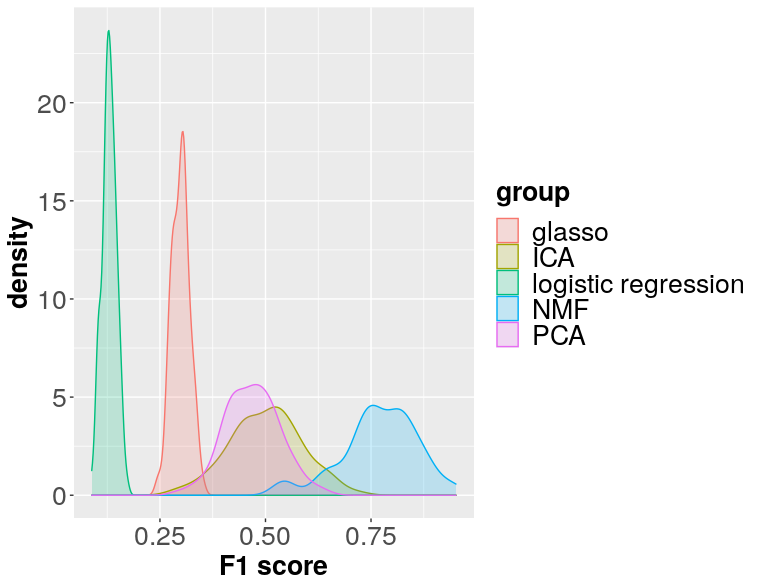
\includegraphics[width=0.5\linewidth]{compare-models}
        \caption{NMF,PCA,ICA,logistic regression,glassoのF1 scoreの密度分布}
        \label{fig:compare-models}
    \end{center}
\end{figure}
\Figref{fig:compare-models}より,NMFの精度が最も高いことが分かる.
NMFの非負制約がデータの生成モデルに合っているためだと思われる.
Glassoとlogistic regressionについては精度が低いが,各窓ごとのニューロンネットワークの活動を反映している可能性があるので,この実験のみで有用性は判断できない.

% \subsection{推定へのネットワーク構造の影響}
% グループ推定へのネットワーク構造の影響を調べるために,1と2のネットワーク構造とグループについて100種類のデータを生成し,NMFの推定精度の比較を行った.
% 人工データは,近いニューロンほどつながりやすい性質をもつので,1の人工データの方がニューロン同士が同期して活動しやすいと思われる.
% ここで,2つのニューロンが同期するとは,一方のニューロンが発火してからごく短い間にもう一方のニューロンが発火する状態が続くことである.
% 実験結果を\Figref{fig:same-exc}~\ref{fig:diff-inh}に示す.
% \begin{figure}[htbp]
%     \begin{center}
%         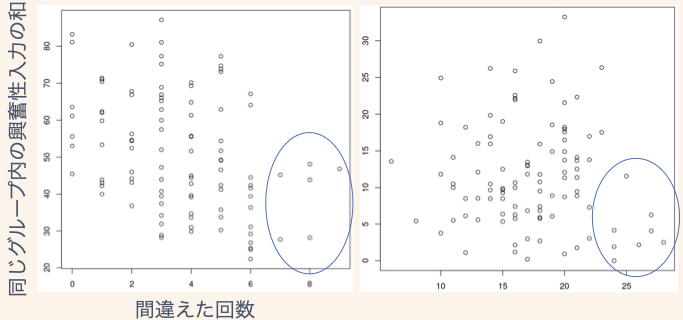
\includegraphics[width=\linewidth]{same-exc}
%         \caption{データ1と2について,ニューロンごとの間違えた回数と同じグループからの興奮性入力の和の関係}
%         \label{fig:same-exc}
%     \end{center}
% \end{figure}
% \begin{figure}[htbp]
%     \begin{center}
%       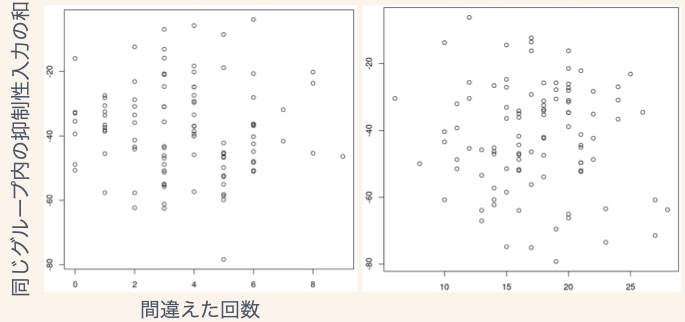
\includegraphics[width=\linewidth]{same-inh}
%         \caption{データ1と2について,ニューロンごとの間違えた回数と同じグループからの抑制性入力の和の関係}
%         \label{fig:same-inh}
%     \end{center}
% \end{figure}
% \begin{figure}[htbp]
%     \begin{center}
%         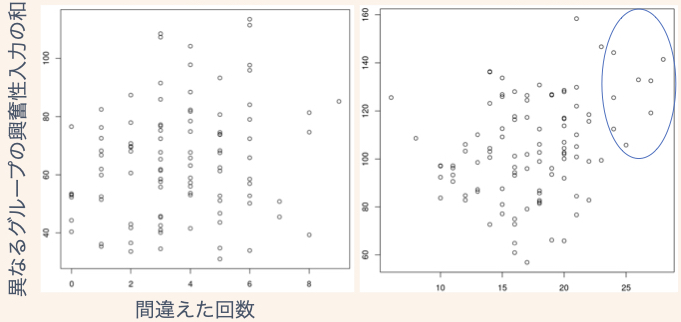
\includegraphics[width=\linewidth]{diff-exc}
%         \caption{データ1と2について,ニューロンごとの間違えた回数と異なるグループからの興奮性入力の和の関係}
%         \label{fig:diff-exc}
%     \end{center}
% \end{figure}
% \begin{figure}[htbp]
%     \begin{center}
%         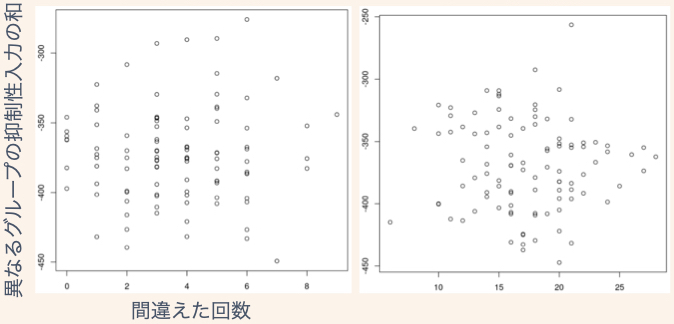
\includegraphics[width=\linewidth]{diff-inh}
%         \caption{データ1と2について,ニューロンごとの間違えた回数と異なるグループからの興奮性入力の和の関係}
%         \label{fig:diff-inh}
%     \end{center}
% \end{figure}
% \Figref{fig:same-inh},\Figref{fig:diff-inh}より,抑制性の入力は間違える回数には影響しないと思われる.
% \Figref{fig:same-exc}より,同じグループからの興奮性入力が小さいと間違えやすいと言える.
% \Figref{fig:diff-exc}より,データ2で間違える回数が多かったニューロンは異なるグループからの興奮性入力が大きかった.
% データ2ではデータ1よりも近いニューロンが異なるグループに所属する割合が多い.
% そのため,異なるグループからの興奮性入力と間違える回数の関係が強く出たと思われる.
% 
% 他にも推定へのネットワーク構造の影響の調査を試みたが,はっきりとした結果は得られなかった.

\subsubsection{バギングの効果}
ブートストラップ法で$\bar{A}(X,\mathcal{K})$を推定する有用性を確認するために,1回NMFを行って$\hat{A}$を推定した結果,30回初期値を変えて$\hat{A}$を推定して平均を取った結果,30回ブートストラップを行って$\bar{A}$を推定した結果のF1 scoreを~\Figref{fig:once-init-boot}に示す.
NMFの基底数は真の基底数10を用いた.
\Figref{fig:once-init-boot}より,ブートストラップを行った方が精度が高くなることがわかる.

\subsubsection{モデル平均の精度}
モデル平均を行うことでそれほど精度は落ちないことを検証するために,基底数別に推定された$\bar{A}$とモデル平均をとった$\bar{A}$のF1 scoreを算出した.
その結果を\Figref{fig:f1all}に示す.
これより,真の基底数周りの$\bar{A}$の平均をとることで精度は保たれることがわかる.

\begin{figure}[htbp]
    \begin{minipage}{0.5\hsize}
			\begin{center}
					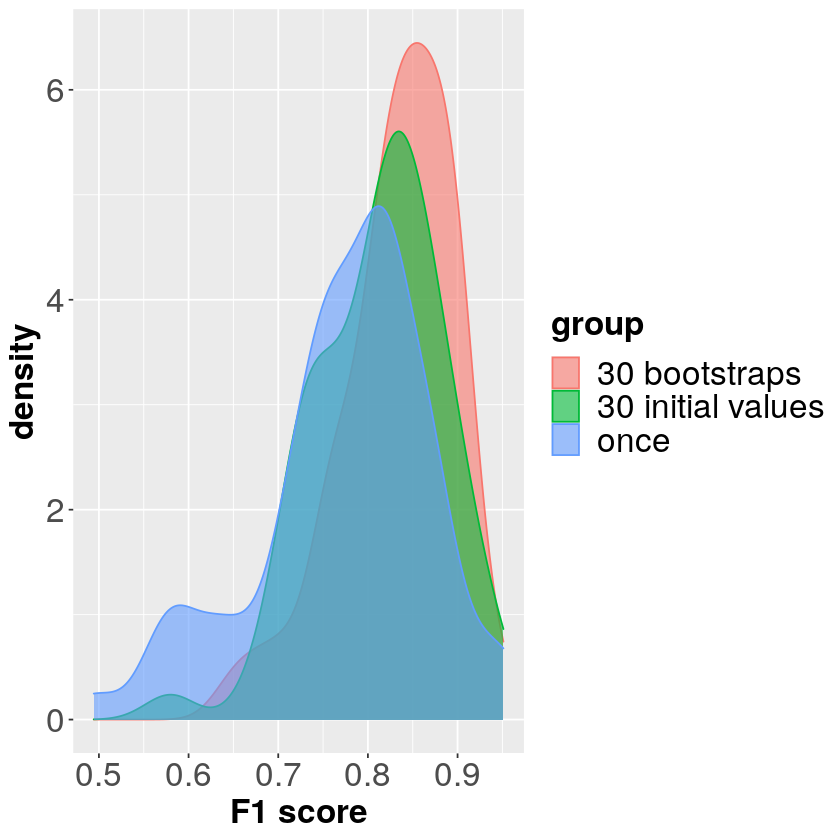
\includegraphics[width=\hsize]{once-init-boot}
					\caption{NMFを1回行った時の$\hat{A}(X,10)$,30回初期値を変えた$\hat{A}(X,10)$の平均,30回ブートストラップを行った$\bar{A}(X,\mathcal{K}); \mathcal{K} = {10}$それぞれのF1 scoreの分布.}
					\label{fig:once-init-boot}
			\end{center}
		\end{minipage}
    \begin{minipage}{0.5\hsize}
			\begin{center}
					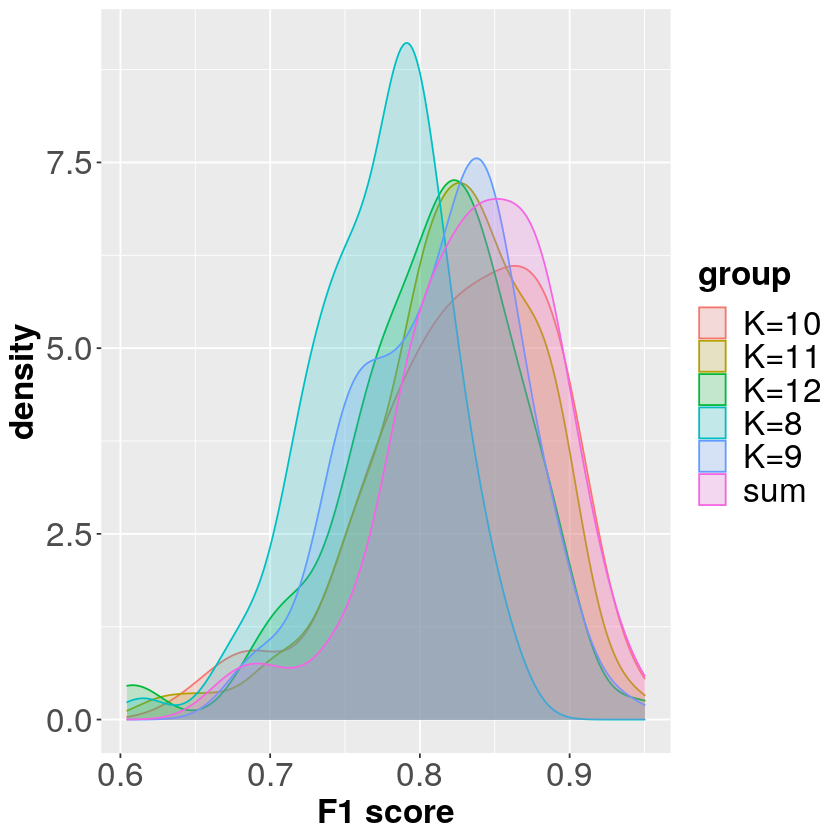
\includegraphics[width=\hsize]{f1all}
					\caption{基底数ごとにブートストラップを行った時の$\bar{A}(X,{K})$のF1 scoreと全ての基底数についてモデル平均をとった$\bar{A}(X,\mathcal{K})$のF1 scoreの分布.}
					\label{fig:f1all}
			\end{center}
		\end{minipage}
\end{figure}

\subsubsection{NMFの基底数}
NMFの基底数を決める方法をいくつか試した.
人工データ86個についてBrunetらとUbrauらの方法で基底数を決めた時に各基底数が何回選ばれるかを~\Figref{fig:cophenetic}と\Figref{fig:uoi}に示す.
Brunetらの方法では初期値を変化させていたが,本実験ではブートストラップの結果で代用している.
Brunetらの方法では真の基底数10に近い基底数が多く選ばれているが,小さい基底数も選ばれている.
Ubaruらの方法では小さい基底数が選ばれる傾向にあった.

また,1つの人工データについてAICとAICcを計算した結果を~\Figref{fig:aic}と\Figref{fig:aicc}に示す.
AICとAICcは最小となるモデルを選択する情報量基準だが,基底数が大きくなるごとに減少する傾向があった.
他の人工データについても同様の傾向にあった.

\begin{figure}[htbp]
    \begin{minipage}{0.5\hsize}
        \begin{center}
            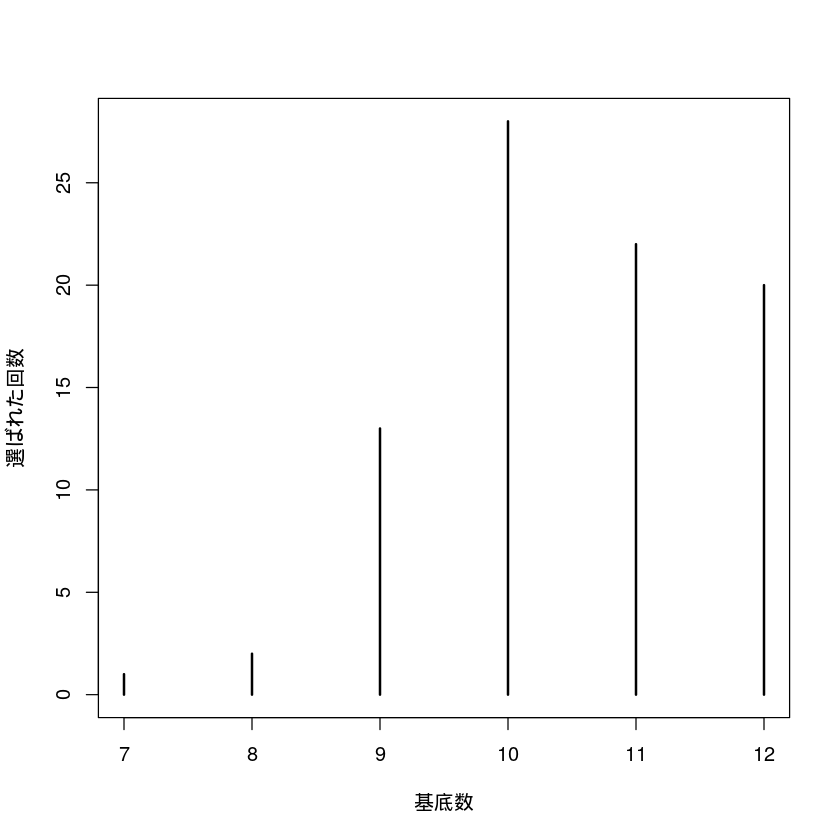
\includegraphics[width=\hsize]{cophenetic}
						\caption{Brunetらの方法で基底数を決めた時に各基底数が選ばれた回数(真の基底数は10).}
            \label{fig:cophenetic}
        \end{center}
    \end{minipage}
    \begin{minipage}{0.5\hsize}
        \begin{center}
            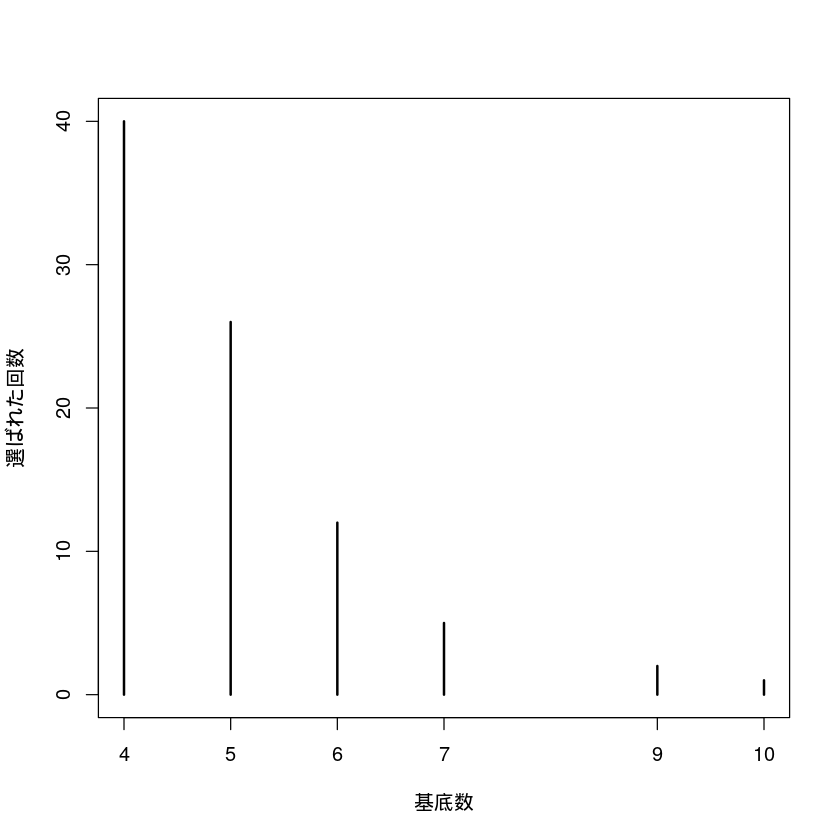
\includegraphics[width=\hsize]{uoi}
						\caption{Ubaruらの方法で基底数を決めた時に各基底数が選ばれた回数(真の基底数は10).}
            \label{fig:uoi}
        \end{center}
    \end{minipage}
\end{figure}
\begin{figure}[htbp]
    \begin{minipage}{0.5\hsize}
        \begin{center}
            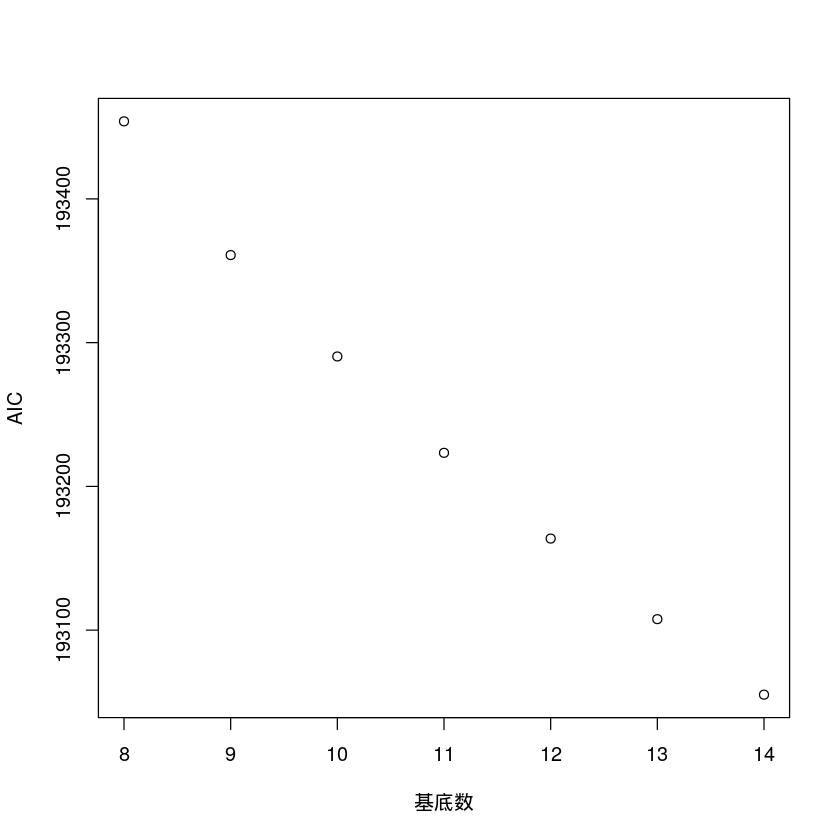
\includegraphics[width=\hsize]{aic}
						\caption{あるデータについてAICを計算した時の結果.}
            \label{fig:aic}
        \end{center}
    \end{minipage}
    \begin{minipage}{0.5\hsize}
        \begin{center}
						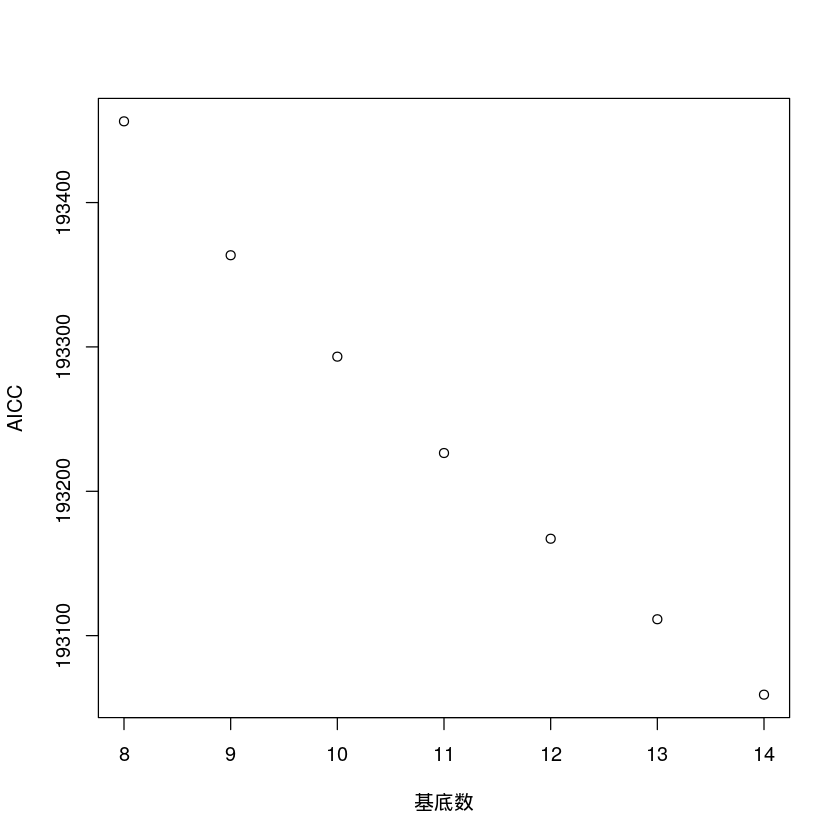
\includegraphics[width=\hsize]{aicc}
						\caption{あるデータについてAICc\cite{Symonds2011}を計算した時の結果.}
            \label{fig:aicc}
        \end{center}
    \end{minipage}
\end{figure}

\subsection{$\bar{A}$のクラスタリングに関する実験}
得られた類似度$\bar{A}$についてスペクトラルクラスタリングを行い,精度を確かめる.
比較手法には\cite{Molter2018}で性能の良かったICA-CSを用いる.
ICA-CSのパラメータは論文中で推奨されていたものを用いた.
また,相関行列を$k$近傍法($k=20$)で隣接行列にしたものと$\varepsilon$近傍法($\varepsilon$は相互相関行列の上から20[\%]の値)で隣接行列にしたものとも比較を行う.
実データを扱う際には$k$や$\varepsilon$をどう設定すればいいか分からない.
また,グループ内のニューロン数に大きな差がある場合は$k$近傍法ではうまく推定できないことが考えられる.
今回は比較のために$k$と$\varepsilon$の値を有利だと思われる値にした.

\subsubsection{クラスタリング実験}
人工データ実験の設定を\Tabref{tab:exp2param1}に,NMFの設定を\Tabref{tab:exp2param2}に示す.
\begin{table}[htb]
  \center
  \begin{tabular}{c|c} \hline
		シミュレーション時間 & 900[s]\\
		グループの活動時間 & 5[s] \\
		グループの活動可能回数 & 60, 30 \\
		$W$の種類 & 2番目 \\
		$Ne_{plus}$ & 0.5 \\
		$Ni_{plus}$ & 0.2\\
		シミュレーション回数 & 50\\ \hline
  \end{tabular}
  \caption{人工データの設定}
  \label{tab:exp2param1}
\end{table}

\begin{table}[htb]
  \center
  \begin{tabular}{c|c} \hline
		1回の結果を出すNMFの回数 & 20 \\
		基底数 & 8 - 12 \\
		ブートストラップサンプル数 & 30 \\
		ブートストラップ方法 & 列のサンプリング \\ \hline
  \end{tabular}
  \caption{NMFの設定}
  \label{tab:exp2param2}
\end{table}
作成した人工データの種類を\Tabref{tab:art_dat}に示す.
900[s]のシミュレーションではニューロングループは5[s]活動する機会が180回与えられる.
その全てでいずれかのグループを活動させるわけではなく,活動できる時間帯をランダムに決める.
人工データnon-active120では活動可能回数を60回,non-active150では活動可能回数を30回とした.
1回の活動の機会ではグループは1つか2つ活動できる.
人工データはnon-active120をベースとして,グループに所属しないニューロンがある場合の提案アプローチの効果を確かめるためにnon-active120-0groupを設計している.
また,活動回数を減らした時の提案アプローチの効果を確認するためにnon-active150を設計している.

\begin{table}[htb]
  \center
  \begin{tabular}{|c|ccc|} \hline
		人工データの種類 & グループ数 &
		\begin{tabular}{c}
			活動回数\\(180回中)
		\end{tabular}
		& 特徴 \\ \hline
		non-active120 & 10 & 60 &
		\begin{tabular}{c}
			ニューロンは必ず\\1つのグループに所属する
		\end{tabular}\\ \hline
		non-active120-0group & 9 & 60 &
		\begin{tabular}{c}
			ニューロンの約10\%は\\グループに所属しない
		\end{tabular}\\ \hline
		non-active150 & 10 & 30 &
		\begin{tabular}{c}
			ニューロンは必ず\\1つのグループに所属する
		\end{tabular}\\ \hline
  \end{tabular}
  \caption{人工データの種類}
  \label{tab:art_dat}
\end{table}

評価方法は5つ用いる.
1つ目は,$\bar{A}$をそのままクラスタリングしてBMSを計算する.
残りの4つは,ニューロンを2種類の閾値で除去し,それぞれ2種類の方法でBMSを評価する.
提案アプローチでは,ニューロン$i$が他の全てのニューロンと同じグループになる確率が閾値を下回った場合にニューロン$i$を取り除くが,その閾値を0.5と0.6として設定した.
ニューロンが取り除かれた場合,$\bar{A}$から該当するニューロンの行と列を削除してクラスタリングを行う.
これらの結果の評価として,真のグループから除去したニューロンを取り除いた場合と取り除かない場合でBMSを計算する.

\Tabref{tab:art_dat}の3種類のデータについて,$\bar{A}$と相関行列のスペクトラルクラスタリング,ICA-CSでクラスタリングを行った.
真のクラスタとのBest Match score(以降BMS)を算出した結果を\Figref{fig:bms}に示す.
相互相関行列に$k$近傍法を用いた場合をcorrelation-k,$\varepsilon$近傍法を用いた場合をcorrelation-$\varepsilon$としている.
提案手法の評価方法は,$\bar{A}$をそのままクラスタリングしたものをproposed-unremove,閾値0.5でニューロンを除去して真のグループから該当ニューロンを取り除いて評価したものをproposed0.5ch,真のグループのまま評価したものをproposed0.5としている.
閾値を0.6にした場合も同じ表記である.
\begin{figure}[htbp]
    \begin{center}
        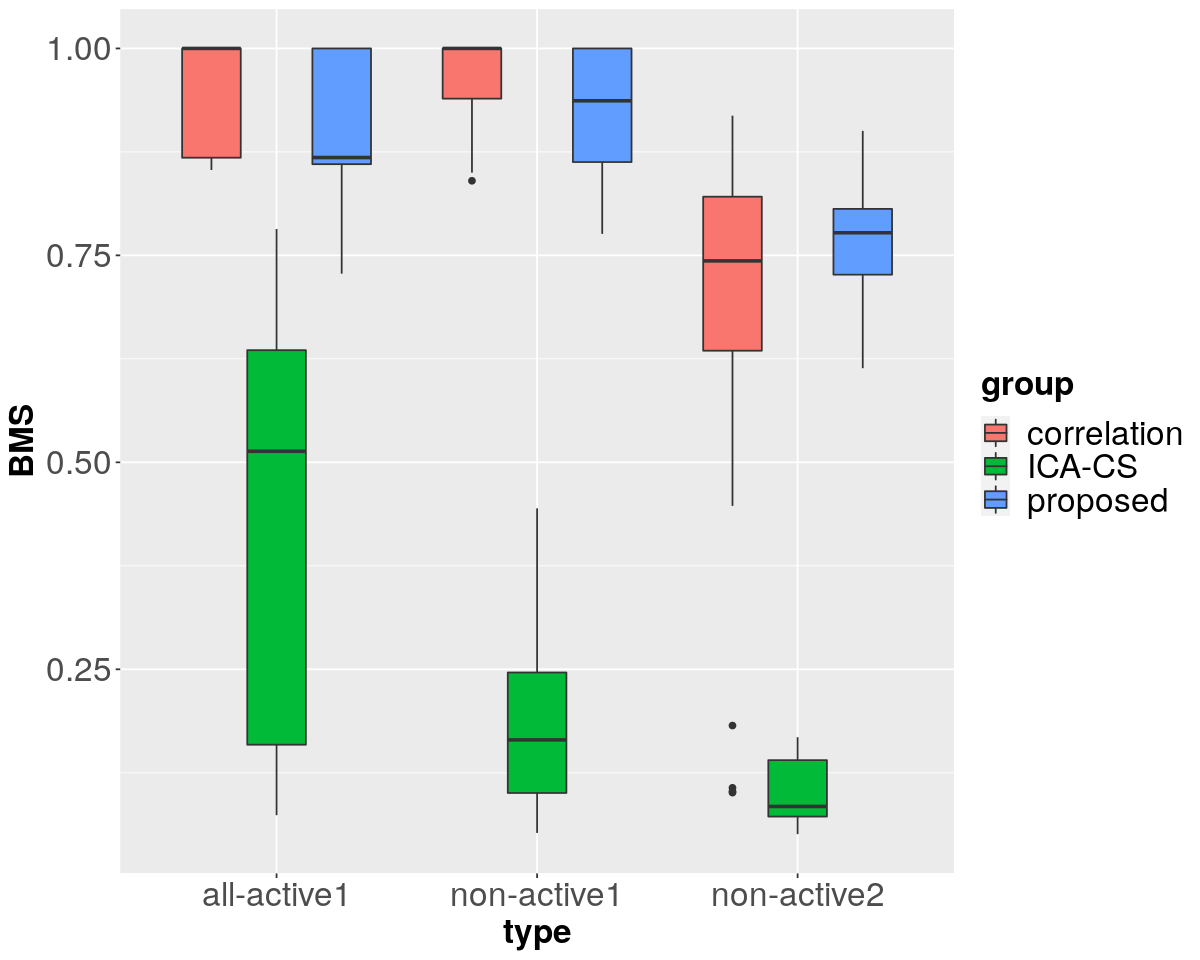
\includegraphics[width=\linewidth]{bms}
        \caption{3種類の人工データについて提案アプローチ,相関行列,ICA-CSでクラスタリングをした結果.}
        \label{fig:bms}
    \end{center}
\end{figure}
ICA-CSは3種類の人工データ全てにおいてBMSが低い.
これは,パラメータが適切ではなく多くのニューロンがクラスタに属していないからだと思われる.
相互相関行列に$\varepsilon$近傍法を用いた場合は$k$近傍法を用いた場合よりBMSが低くなっている.
相互相関行列を閾値で切るとニューロンごとにエッジの数が多いものと少ないものができてしまい,それが影響を与えていると考えられる.
non-active120では,相互相関行列に$k$近傍法を用いた場合の方が提案アプローチよりBMSが高くなっている.
しかし,non-active120-0groupでは提案アプローチより相互相関行列のBMSの下り幅が大きくなっている.
これは,ランダムに活動するニューロンの存在が相互相関行列によるクラスタリングに悪影響を与えているためだと思われる.
グループが活動する時間帯を減らしたnon-active150でも相互相関行列のBMSの下り幅が提案アプローチよりも大きい.
ニューロンがグループに依らずランダムに活動する時間が多いことが相互相関行列によるクラスタリングに悪影響を与えていると思われる.
これより,ランダムに活動するニューロン数や全ニューロンがランダムに活動する時間に対して,提案アプローチの方が相互相関行列よりもロバストだと考えられる.

人工データnon-active120-0groupで閾値0.5と0.6で取り除いたニューロンのprecisionとrecallをそれぞれ\Figref{fig:prerec05}と\Figref{fig:prerec06}に示す.
プロットの大きさは,その座標にある点の数を表している.
プロットの色は,そのデータ内で取り除かれたニューロン数を示している.
閾値0.5の方が取り除いている数は少ないがprecisionは高い.
また,\Figref{fig:bms}でもproposed0.5の方がproposed-unremoveよりBMSが高い.
それに対してproposed0.6のBMSはproposed-unremoveより下がっている.
よって,閾値は0.6より0.5を採用すべきである.
\begin{figure}[htbp]
    \begin{minipage}{0.5\hsize}
			\begin{center}
					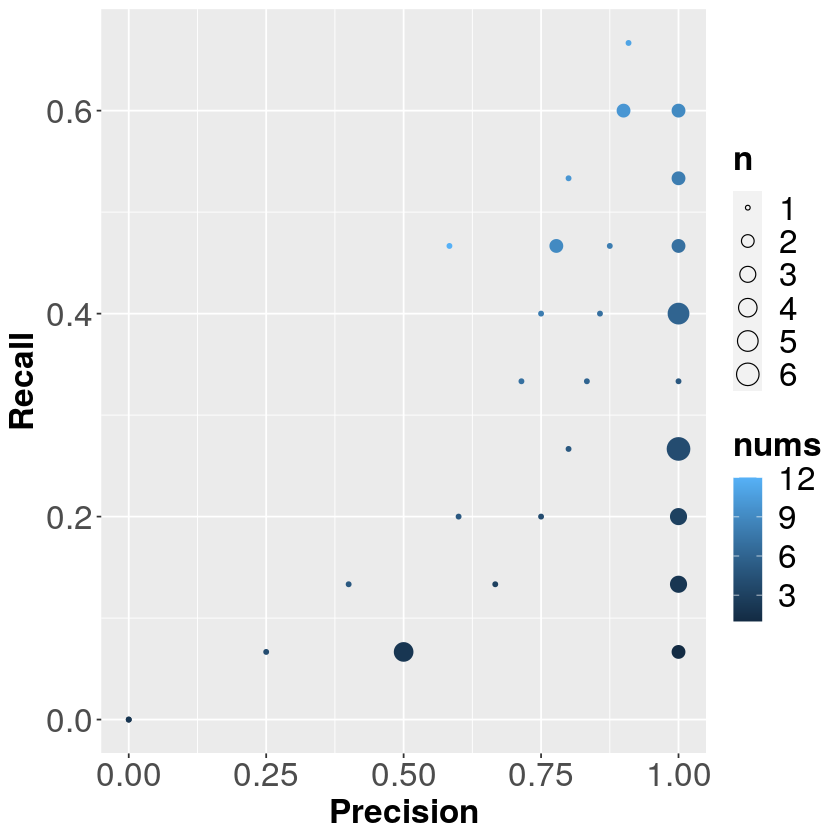
\includegraphics[width=\hsize]{prerec05}
					\caption{non-active120-0groupで閾値0.5でニューロンを切った場合のprecisionとrecall.}
					\label{fig:prerec05}
			\end{center}
		\end{minipage}
    \begin{minipage}{0.5\hsize}
			\begin{center}
					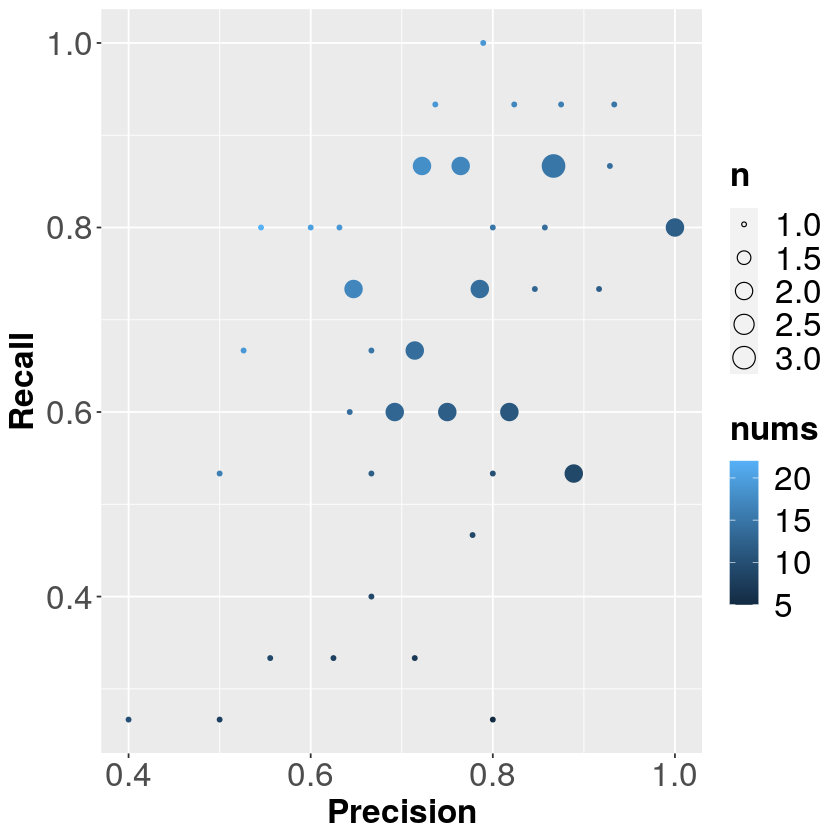
\includegraphics[width=\hsize]{prerec06}
					\caption{non-active120-0groupで閾値0.6でニューロンを切った場合のprecisionとrecall.}
					\label{fig:prerec06}
			\end{center}
		\end{minipage}
\end{figure}

固有値ギャップと大津の二値化によって推定されたクラスタ数を比較する.
3種類の人工データそれぞれについて相互相関行列で推定されたクラスタ数と提案アプローチで推定されたクラスタ数を\Figref{fig:non-active120-ks}〜\ref{fig:non-active150-ks}に示す.
提案アプローチの方が安定して真のクラスタ数を当てられていることがわかる.
\Figref{fig:bms}でcorrelation-kのBMSの低さやばらつきの大きさは,推定されたクラスタ数によるばらつきも関係していると思われる.
\begin{figure}[htbp]
    \begin{minipage}{0.5\hsize}
			\begin{center}
					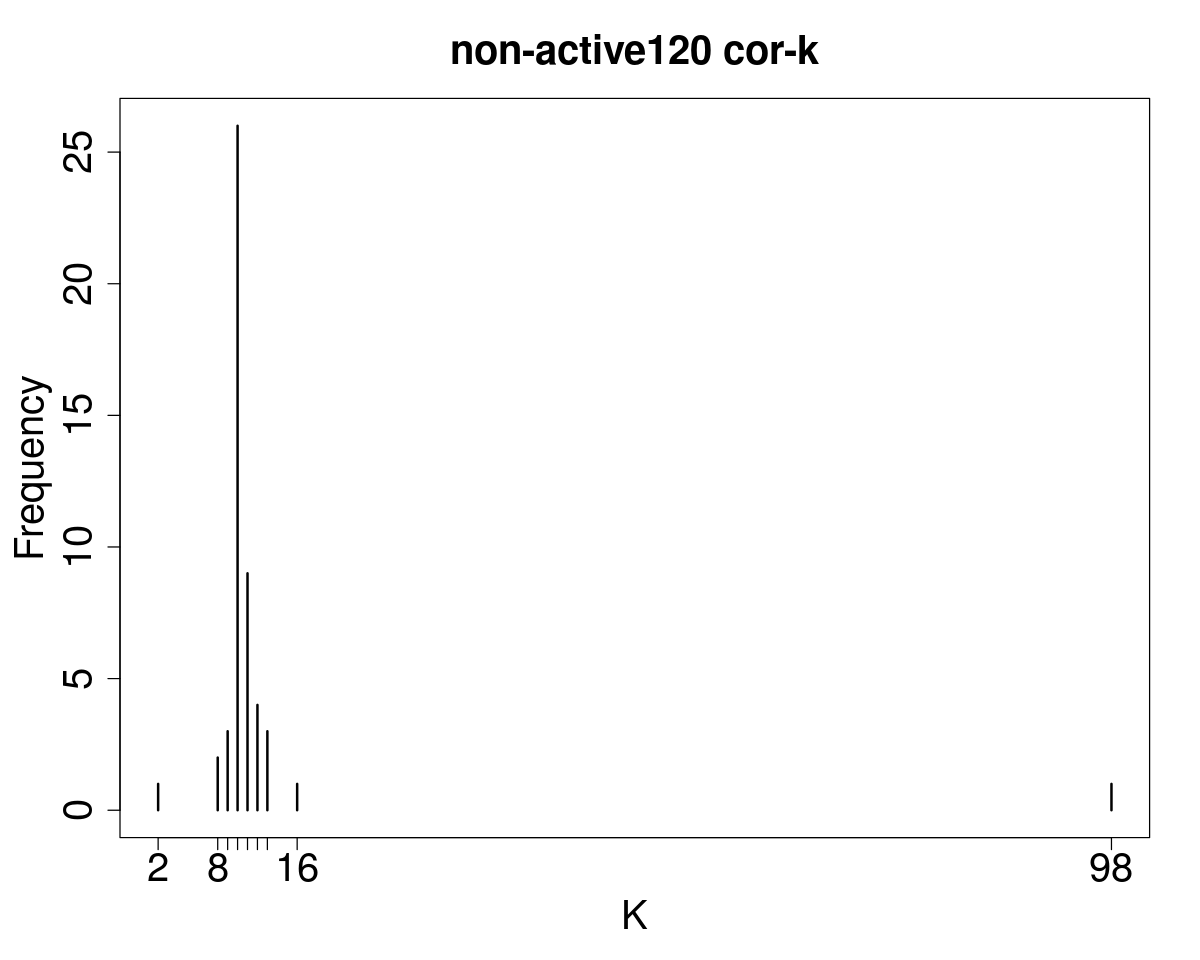
\includegraphics[width=\hsize]{non-active120-corks}
			\end{center}
		\end{minipage}
    \begin{minipage}{0.5\hsize}
			\begin{center}
					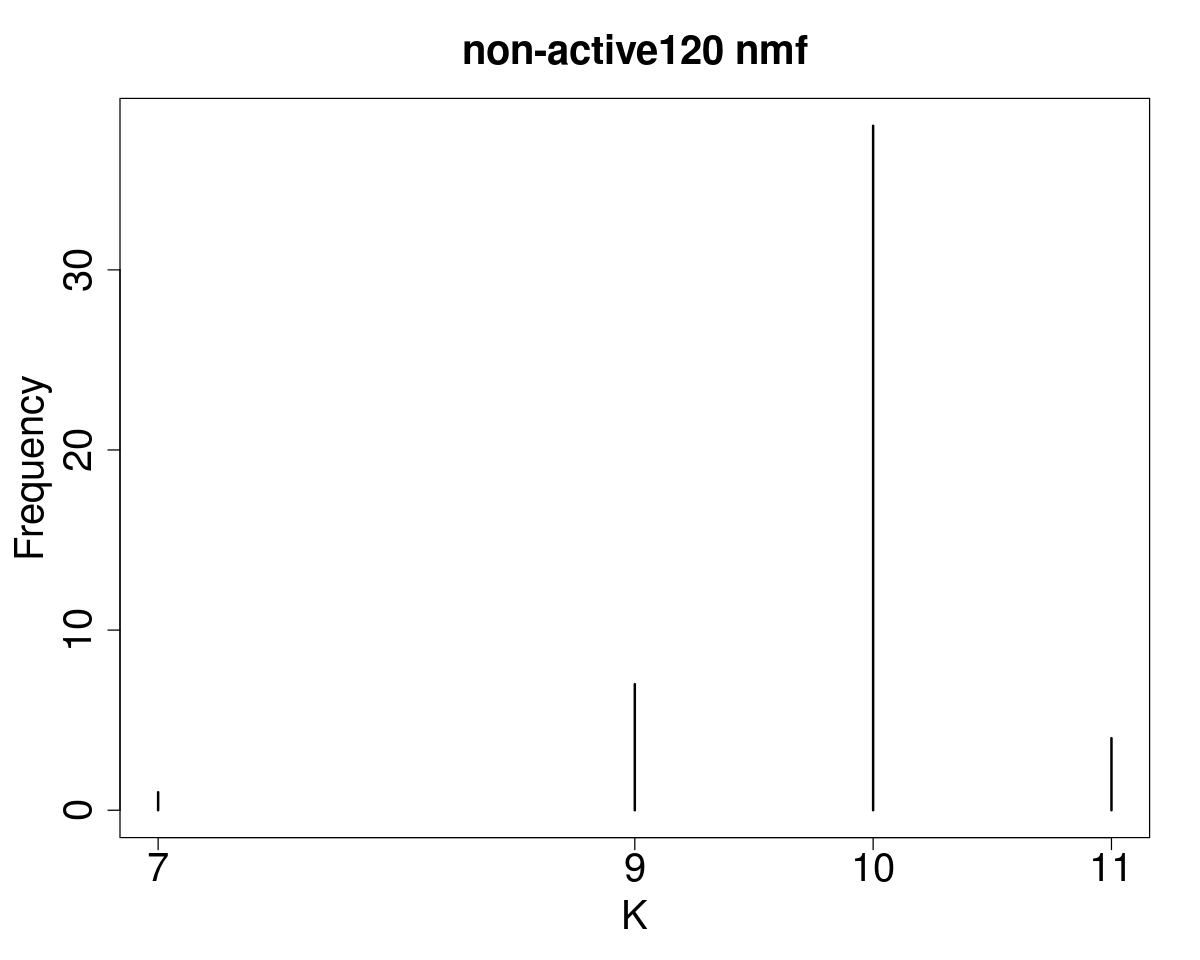
\includegraphics[width=\hsize]{non-active120-nmfks}
			\end{center}
		\end{minipage}
	\caption{non-active120で推定されたクラスタ数.左は相互相関行列に$k$近傍法を用いた場合.右は提案アプローチでニューロン除去しなかった場合.真のクラスタ数は10.}
	\label{fig:non-active120-ks}
\end{figure}
\begin{figure}[htbp]
    \begin{minipage}{0.5\hsize}
			\begin{center}
					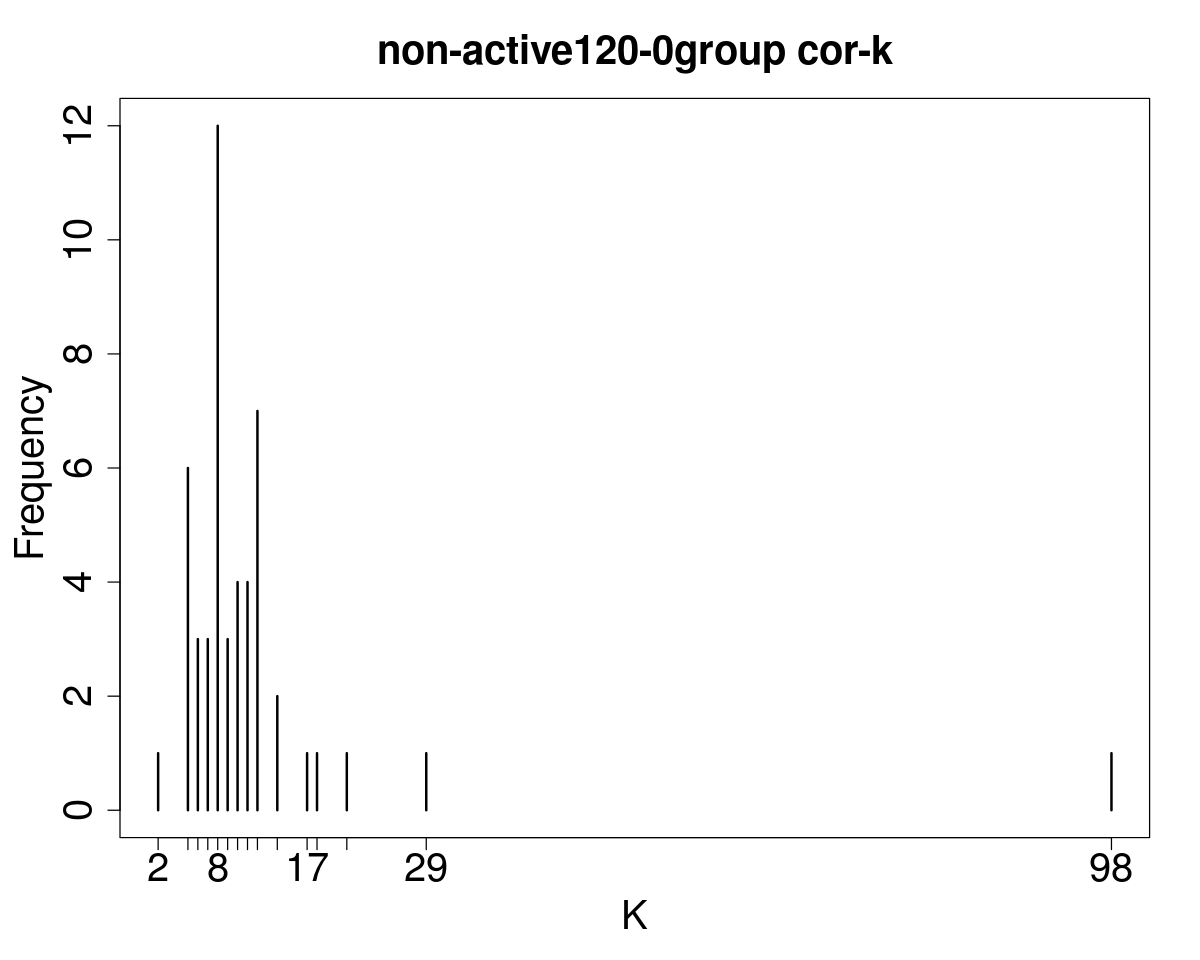
\includegraphics[width=\hsize]{non-active120-0group-corks}
			\end{center}
		\end{minipage}
    \begin{minipage}{0.5\hsize}
			\begin{center}
					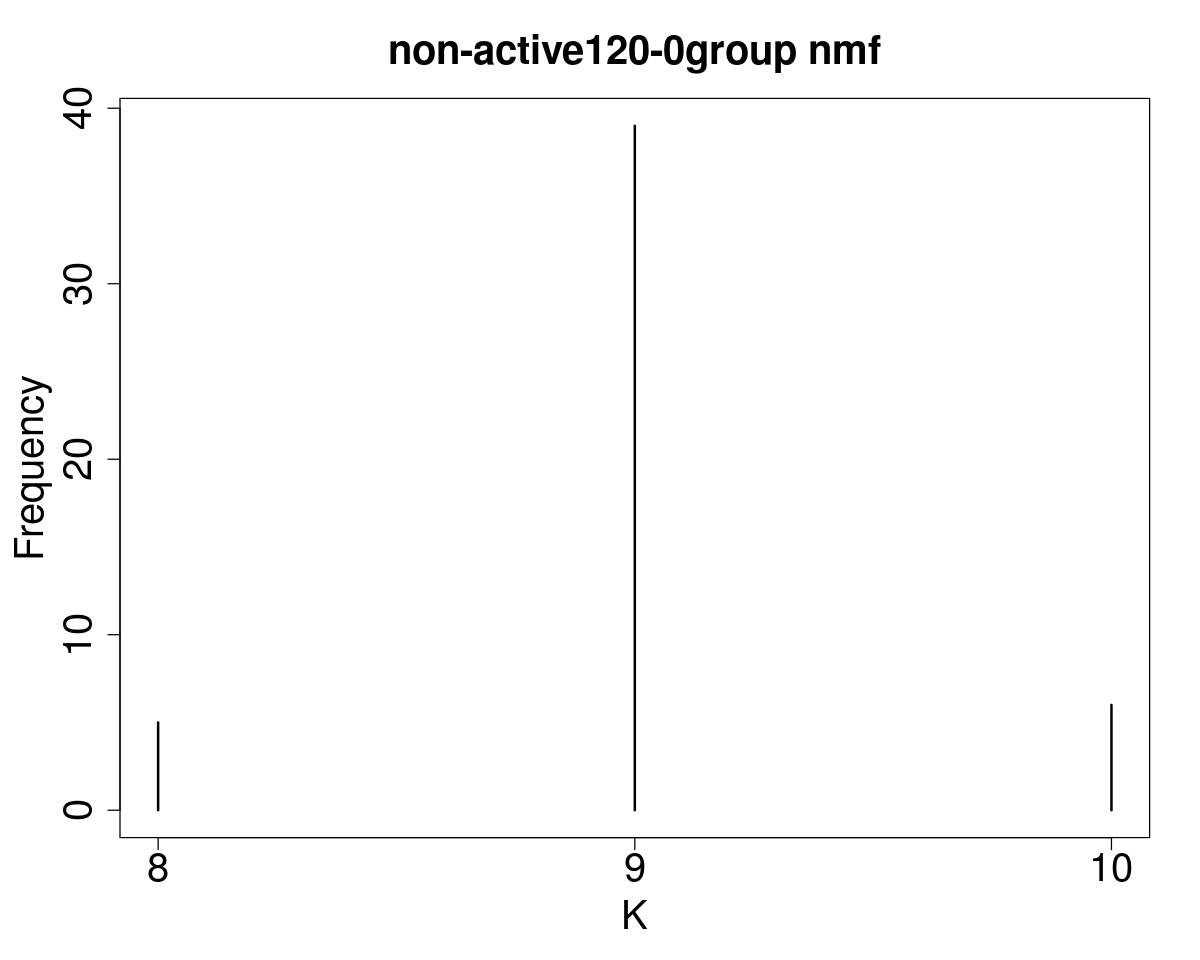
\includegraphics[width=\hsize]{non-active120-0group-nmfks}
			\end{center}
		\end{minipage}
	\caption{non-active120-0groupで推定されたクラスタ数.左は相互相関行列に$k$近傍法を用いた場合.右は提案アプローチで閾値0.5でニューロン除去した場合.真のクラスタ数は9.}
	\label{fig:non-active120-0group-ks}
\end{figure}
\begin{figure}[htbp]
    \begin{minipage}{0.5\hsize}
			\begin{center}
					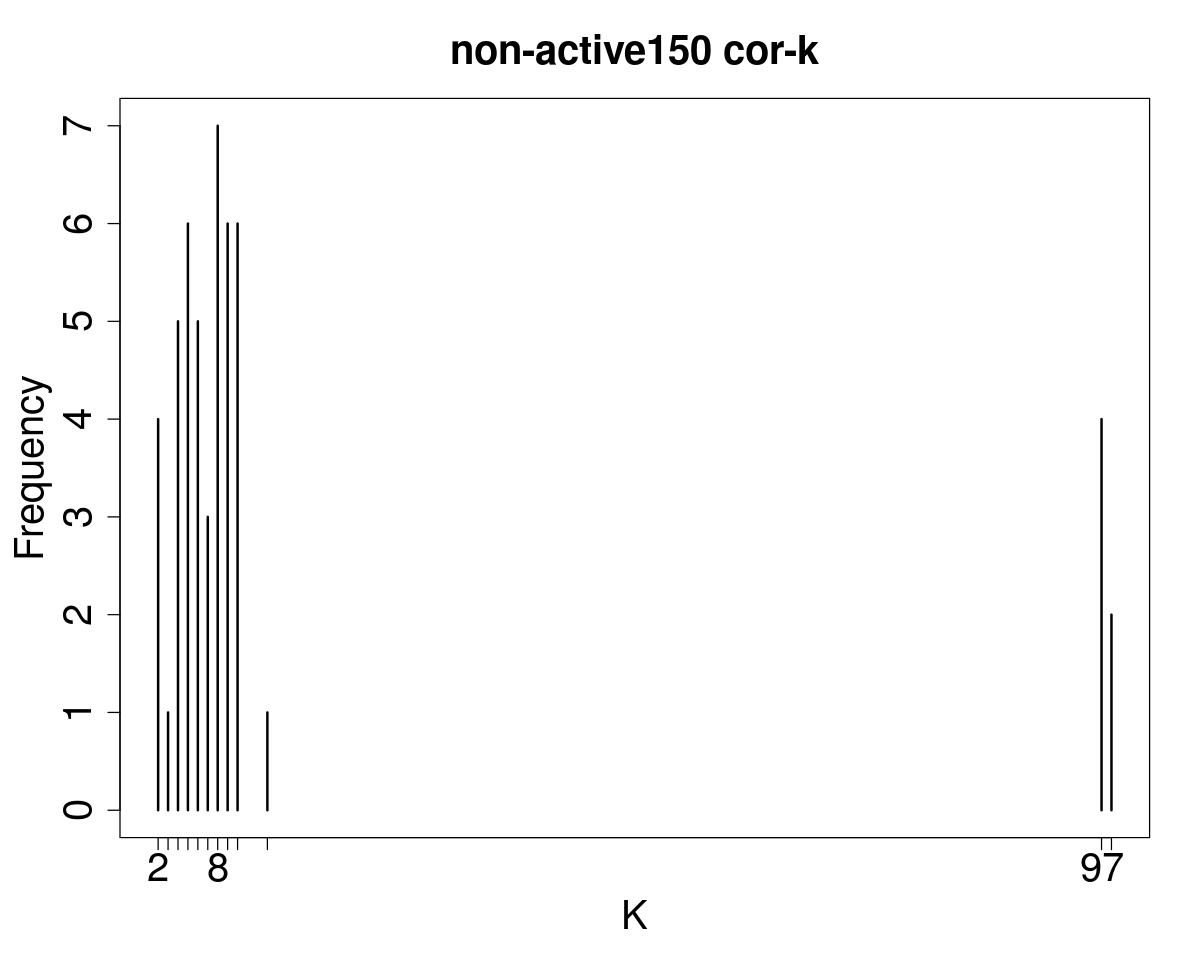
\includegraphics[width=\hsize]{non-active150-corks}
			\end{center}
		\end{minipage}
    \begin{minipage}{0.5\hsize}
			\begin{center}
					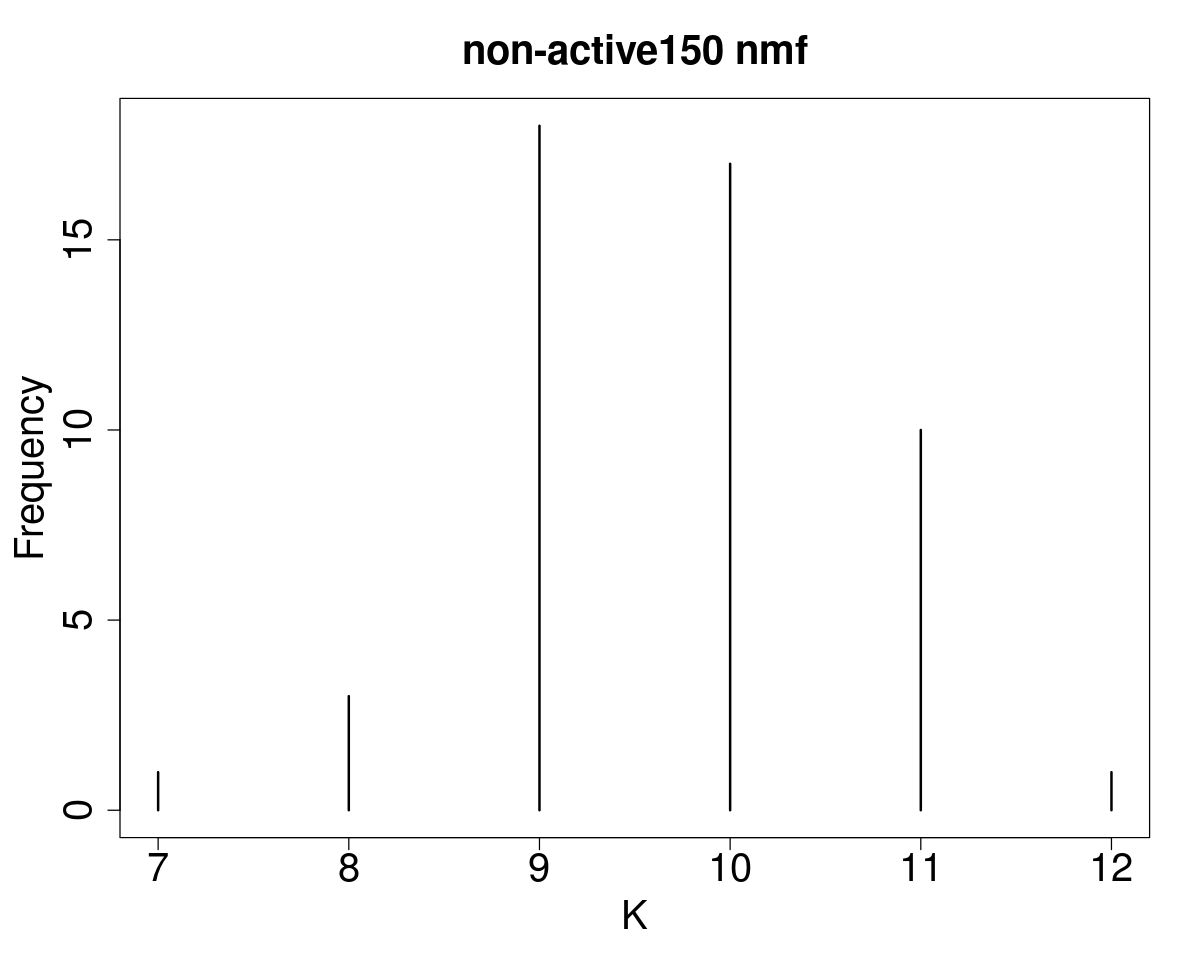
\includegraphics[width=\hsize]{non-active150-nmfks}
			\end{center}
		\end{minipage}
	\caption{non-active150で推定されたクラスタ数.左は相互相関行列に$k$近傍法を用いた場合.右は提案アプローチでニューロン除去しなかった場合.真のクラスタ数は10.}
	\label{fig:non-active150-ks}
\end{figure}

\subsubsection{グループの活動時間数に対する提案アプローチのロバスト性}
グループの活動時間数に対して提案アプローチの方が相互相関行列よりもロバストかを確認するための実験を行った.
人工データ実験の設定を\Tabref{tab:exp3param1}に示す.
グループは100回活動する機会があるが,その中で活動時間帯を70,60,50,40回と減らした4種類の人工データを用いた.
\begin{table}[htb]
  \center
  \begin{tabular}{c|c} \hline
		シミュレーション時間 & 100[s]\\
		グループの活動時間 & 1[s] \\
		グループの活動可能回数 & 40, 50, 60, 70 \\
		$W$の種類 & 2番目 \\
		$Ne_{plus}$ & 0.8 \\
		$Ni_{plus}$ & 0.4\\
		シミュレーション回数 & 50\\ \hline
  \end{tabular}
  \caption{人工データの設定}
  \label{tab:exp3param1}
\end{table}

提案アプローチと相互相関行列のクラスタリング結果を\Figref{fig:bms2}に示す.
前節の実験よりもシミュレーション時間とグループの活動時間を短くしたため,全体的にBMSが低くなっている.
全ての人工データにおいて提案アプローチのBMSの分散の方が小さい.
グループの活動回数が多いnon-active30では相互相関行列のBMSの中央値の方が高いが,グループの活動回数が少ないnon-active60では提案アプローチのBMSの中央値の方が高くなっている.
これより,活動回数が少ない方が提案アプローチの方がロバストだと考えられ,\Figref{fig:bms}でも同じことが起こっていると考えられる.
\begin{figure}[htbp]
    \begin{center}
        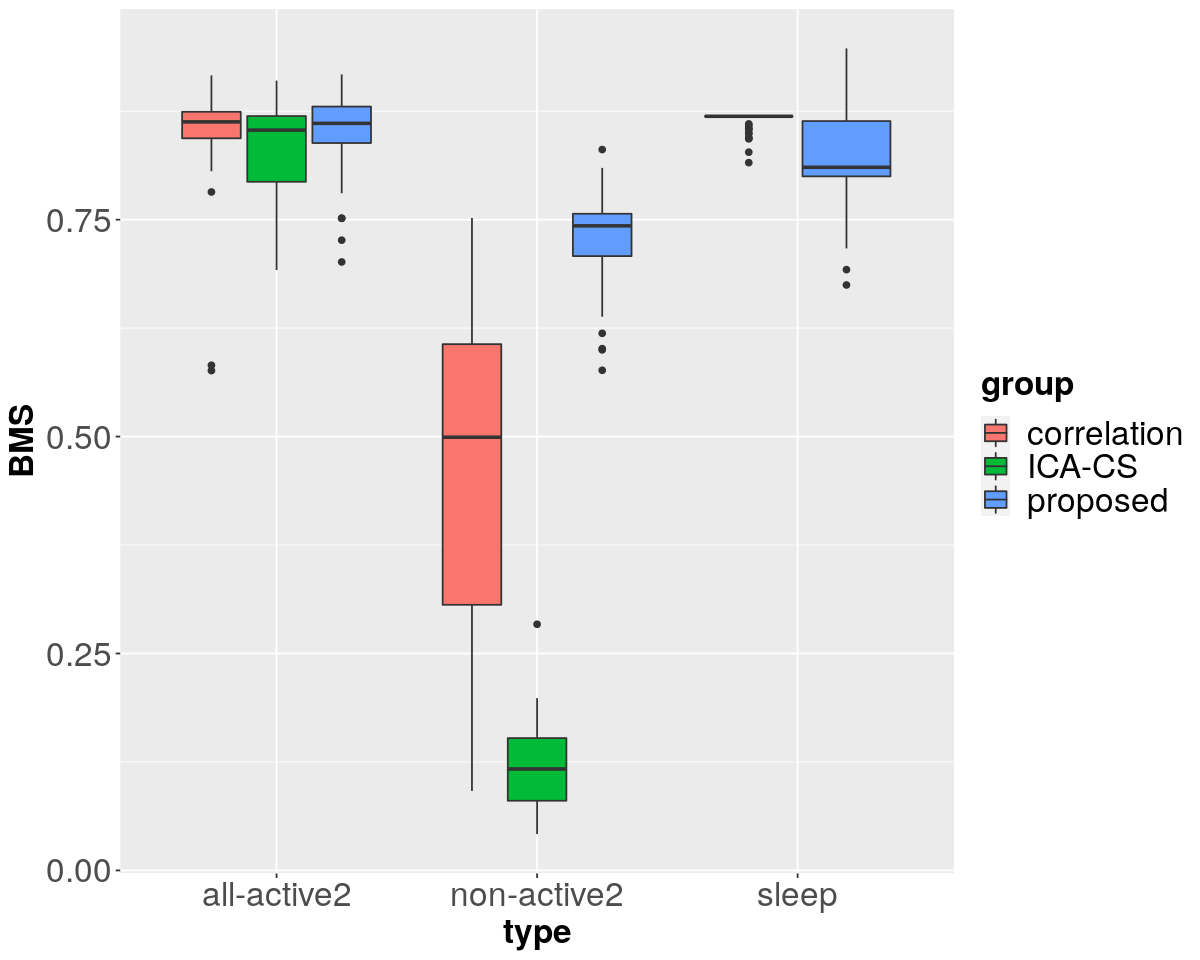
\includegraphics[width=\linewidth]{bms2}
        \caption{4種類の人工データについて提案アプローチと相関行列でクラスタリングをした結果.}
        \label{fig:bms2}
    \end{center}
\end{figure}

\subsubsection{モデル平均の効果}
モデル平均の効果を確かめるため,\Tabref{tab:art_dat}のnon-active120の人工データについて基底数が1つの場合と5つモデル平均した場合を比較した.
基底数が1つの場合は$\mathcal{K} = \{8\}, \cdots, \{22\}$として$\bar{A}$を求め,スペクトラルクラスタリングを行った.
その時のBMSを\Figref{fig:bms_ks}に示す.
基底数が5つの場合は$\mathcal{K} = \{8, \cdots, 12\}, \cdots, \{18, \cdots, 22\}$とした.
その時のBMSを\Figref{fig:bms_means}に示す.
また,それぞれの推定クラスタ数を\Figref{fig:clst_nums_ks}と\Figref{fig:clst_nums_means}に示す.
\Figref{fig:bms_ks}の基底数8のBMSより\Figref{fig:bms_means}の基底数8から12までをモデル平均した時のBMSの方が高いことがわかる.
\Figref{fig:bms_ks}の基底数22の場合も同様に\Figref{fig:bms_means}の基底数18から22のモデル平均の方がBMSが高い.
しかし,\Figref{fig:bms_ks}の基底数18のBMSより良くなっているとは言えない.
あくまでもモデル平均は,真から最も遠い基底数のBMSより良くなるだけであり,リスク回避の役割が大きい.
推定クラスタ数についても同様のことがいえる.

\begin{figure}[htbp]
    \begin{minipage}{0.5\hsize}
			\begin{center}
					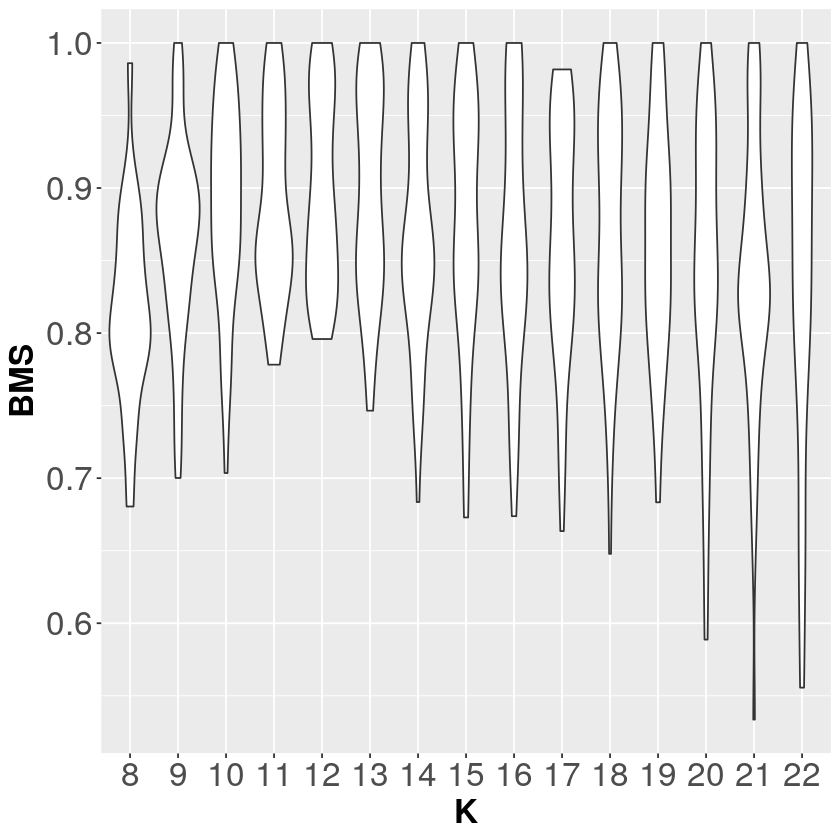
\includegraphics[width=\hsize]{bms_ks}
					\caption{基底数1つの場合のBMSの分布.}
					\label{fig:bms_ks}
			\end{center}
		\end{minipage}
    \begin{minipage}{0.5\hsize}
			\begin{center}
					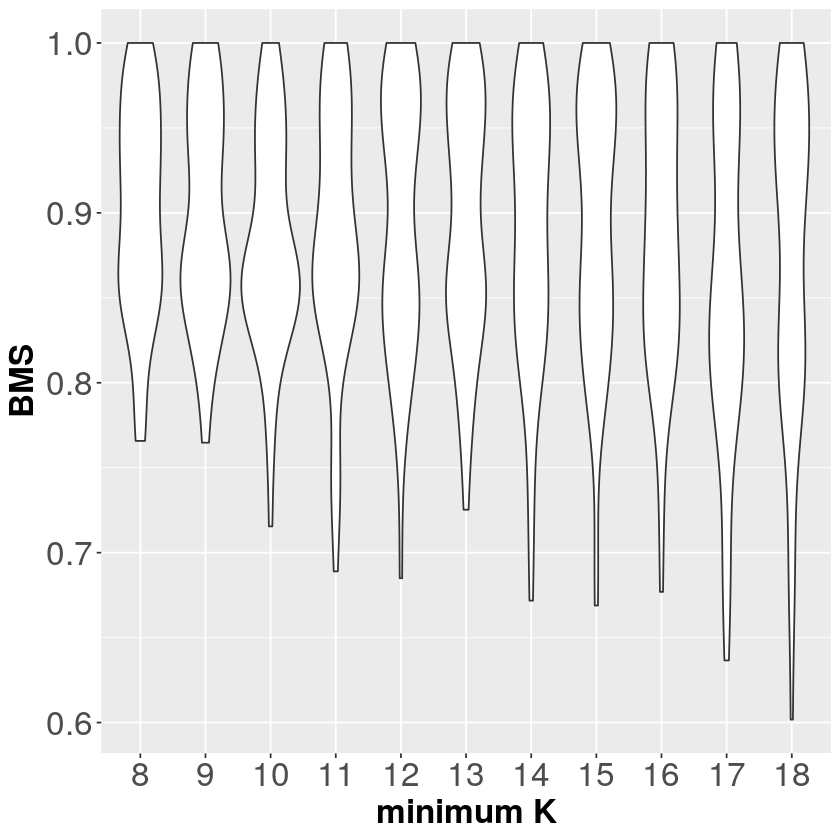
\includegraphics[width=\hsize]{bms_means}
					\caption{基底数5つの場合のBMSの分布.}
					\label{fig:bms_means}
			\end{center}
		\end{minipage}
\end{figure}
\begin{figure}[htbp]
    \begin{minipage}{0.5\hsize}
			\begin{center}
					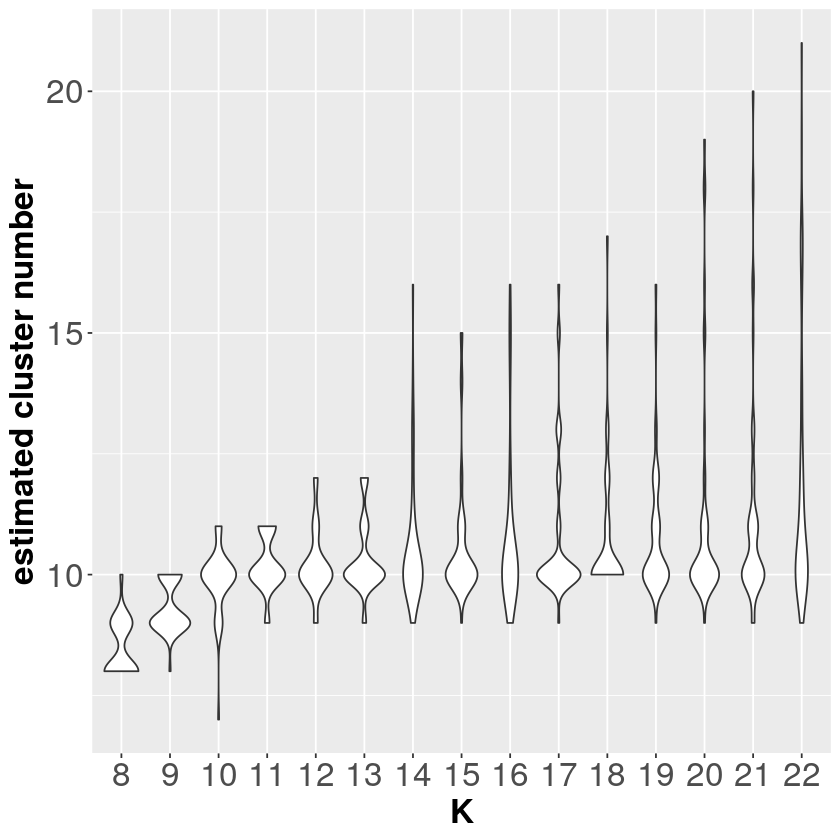
\includegraphics[width=\hsize]{clst_nums_ks}
					\caption{基底数1つの場合の推定クラスタ数の分布.}
					\label{fig:clst_nums_ks}
			\end{center}
		\end{minipage}
    \begin{minipage}{0.5\hsize}
			\begin{center}
					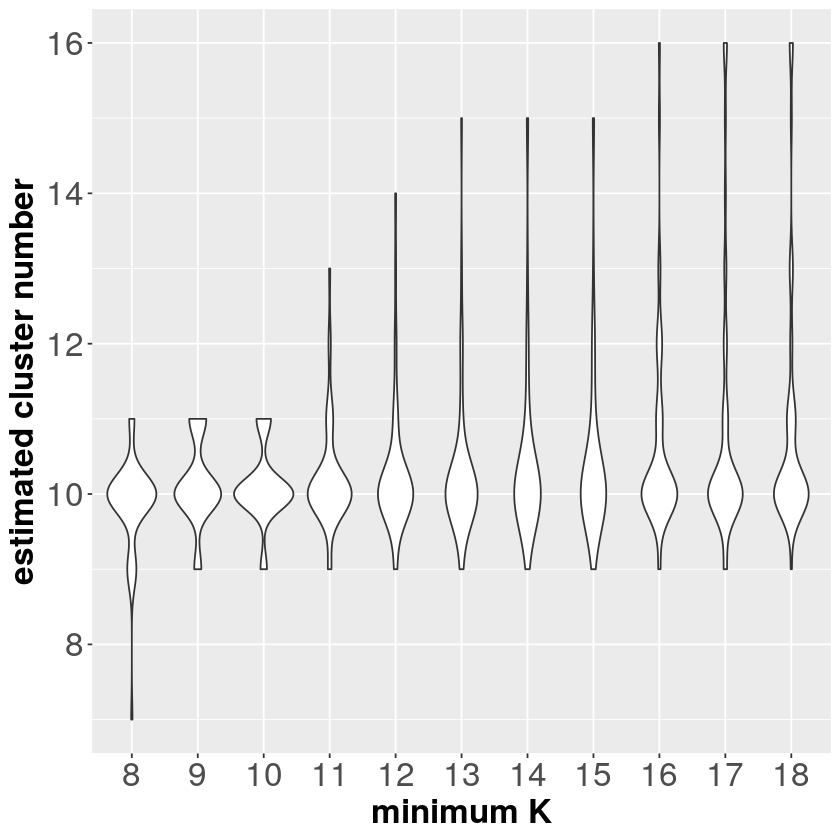
\includegraphics[width=\hsize]{clst_nums_means}
					\caption{基底数5つの場合の推定クラスタ数の分布.}
					\label{fig:clst_nums_means}
			\end{center}
		\end{minipage}
\end{figure}
